\chapter{Implementation}
\label{cha:implementation}

\begin{figure}[ht!]
    \centering
    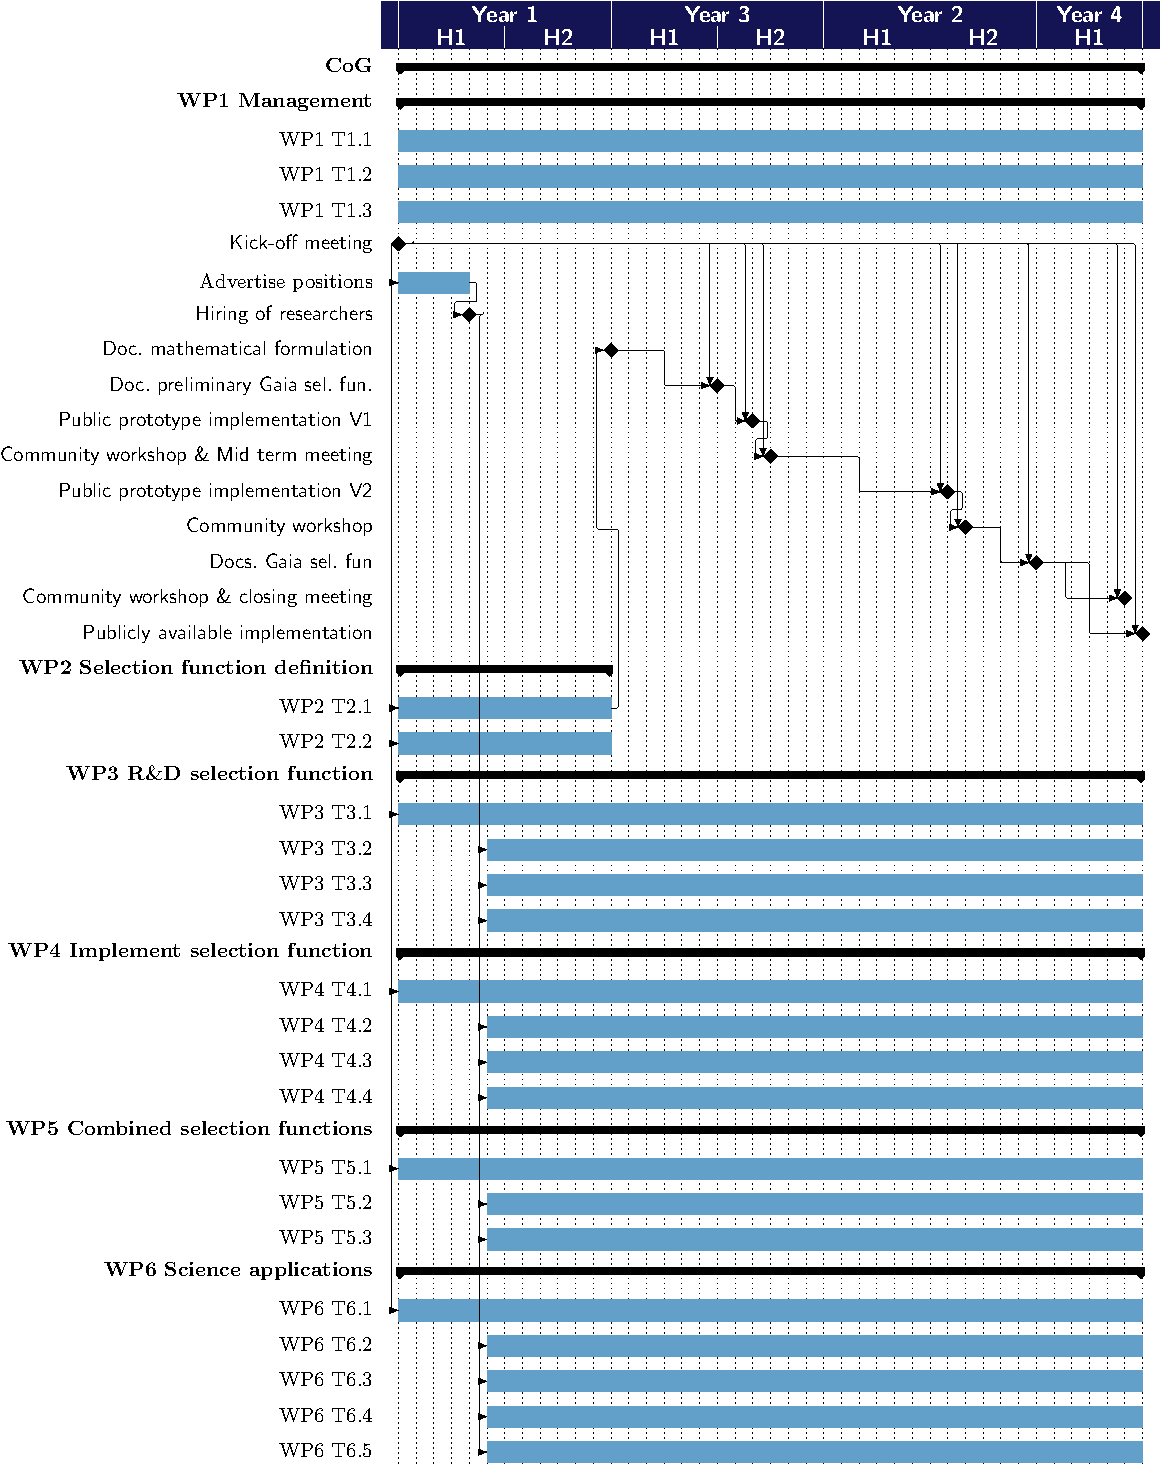
\includegraphics[width=\linewidth]{cog-gantt.pdf}
    \caption{Gantt chart for the {\acro} project.}
    \label{fig:gantt}
\end{figure}

\section{Work plan --- Work packages, deliverables}
\label{sec:work-plan}

\subsection{Overall structure}
\label{sec:wpstructure}



\subsection{Timing of the work package}
\label{sec:wptiming}

The overall work plan is structured as follows:
\begin{itemize}
    \item The first 6 months will be used to recruit the researchers to be funded from this proposal and to carry out the tasks in work package \ref{wp:selfundefinition}. Having a mathematical framework for the selection function in place early on in the project is important for guiding the research and the implementation phases.
    \item During the next three years of the project the efforts in work packages \ref{wp:selfungaia} to \ref{wp:scienceappl} will happen mostly in parallel. This is because the results from each of the four work packages will feed back into the others.
    \item 
 \end{itemize}

\makewplist

%\subsection{Work package description}
%\label{sec:wps}

\tablecaption{Description of work packages}
\begin{supertabular}{p{\textwidth}}
    \omit \tabularnewline
\end{supertabular}
%%%%%%%%%%%%%%%%%%%%%%%%%%%%%%
%  Work Package Description  %
%%%%%%%%%%%%%%%%%%%%%%%%%%%%%%

\begin{workpackage}{Management}
  \label{wp:management} %change and use appropriate description

  %%%%%%%%%%%%%%%%%% TOP TABLE %%%%%%%%%%%%%%%%%%%%%%%%%%%%%
  % Data for the top table
  \wpstart{1} %Starting Month
  \wpend{\duration} %End Month
  \wptype{MGT} %RTD, DEM, MGT, or OTHER
  \wplead{ULEI}

  % Person Months per participant (required, max 7, * for leader)  
  % syntax: \personmonths{Participant number}{value}    (not wp leader)
  %     or  \personmonths{Participant short name}{value} (not wp leader)
  %         \personmonths*{Participant number}{value}    (wp leader)
  % for example:
  \personmonths*{ULEI}{8}
  \personmonths{MPG}{2}
  \personmonths{INAF}{2}
  \personmonths{UCAM}{2}
  \personmonths{NYU}{1}
  \personmonths{MONA}{1}
  % etc.

  \makewptable % Work package summary table

  % Work Package Objectives
  \begin{wpobjectives}
    This package provides the overall scientific coordination and administrative management of \acro\ as described in \secref{sec:management}.
  \end{wpobjectives}

  % Work Package Description
  \begin{wpdescription}
    % Divide work package into multiple tasks.
    % Use \wptask command
    % syntax: \wptask{leader}{contributors}{start-m}{end-m}{title}{description}   

    This work package includes the administrative tasks to fulfil the EC requirements and rules as
    well as the global administrative and coordination tasks inside the consortium, including financial
    management, intellectual property management and project documentation. It also includes the
    coordination with institutions and bodies relevant for the development of the Gaia archive like
    ESA, DPAC and MW-Gaia, as well as the representation of {\acro} in meetings or committees
    related to this coordination.

    \wptask{ULEI}{ULEI}{1}{\duration}{Overall coordination}{
      \label{task:wp1coordinator}
      Overall coordination and administrative management as described above (12 person-months). 
    }
    \wptask{ULEI}{MPG, INAF, UCAM}{1}{\duration}{Scientific coordination}{
      \label{task:wp1others}
      Scientific coordination by the four main partners through the {\acro} Executive Board. As stated in \secref{sec:management}, the partners NYU and MONA will have a standing invitation to meetings of the Executive Board in order to keep communications efficient.
    }    
  \end{wpdescription}
  
  % Work Package Deliverable
  \begin{wpdeliverables}
    % Data for the deliverables and milestones  tables
    % syntax: \deliverable[delivery date]{nature}{dissemination
    % level}{description} 
    %
    % nature: R = Report, DEM = Demonstrator, DEC = Websites, media, etc, OTHER = Other
    % dissemination level: PU = Public, CO = Confidential, CI = CLassified.
    % 
    % \wpdeliverable[date]{R}{PU}{A report on \ldots}

    The deliverables of this work package are the final report for the EC, the consortium agreement
    (\secref{sec:cons_agreement}), the semestral reports for the external advisory board (\secref{sec:mgtdetails}) and the organisation
    of the {\acro} plenary meetings (\secref{sec:procedures}).

    \wpdeliverable[1]{ULEI}{OTHER}{PU}{Kick-off meeting (plenary)}\label{dev:wp1kickoff}
    \wpdeliverable[2]{ULEI}{R}{PU}{Consortium agreement}\label{dev:wp1consortium_agreement}
    \wpdeliverable[6]{ULEI}{R}{PU}{Data management plan}\label{dev:wp1datamanagement}
    \wpdeliverable[6]{ULEI}{R}{PU}{Semestral report 1}\label{dev:wp1sem1}
    \wpdeliverable[12]{ULEI}{R}{PU}{Semestral report 2}\label{dev:wp1sem2}
    \wpdeliverable[18]{ULEI}{R}{PU}{Semestral report 3}\label{dev:wp1sem3}
    \wpdeliverable[21]{ULEI}{OTHER}{PU}{Mid-term meeting (plenary)}\label{dev:wp1midtterm}
    \wpdeliverable[24]{ULEI}{R}{PU}{Semestral report 4}\label{dev:wp1sem4}
    \wpdeliverable[30]{ULEI}{R}{PU}{Semestral report 5}\label{dev:wp1sem5}
    \wpdeliverable[36]{ULEI}{R}{PU}{Semestral report 6}\label{dev:wp1sem6}
    \wpdeliverable[41]{ULEI}{OTHER}{PU}{Community workshop and closing meeting}\label{dev:wp1closing}
    \wpdeliverable[\duration]{ULEI}{R}{PU}{Final report to the EC}\label{dev:wp1finalreport}
  \end{wpdeliverables}

\end{workpackage}


%%% Local Variables:
%%% mode: latex
%%% TeX-master: "proposal-main"
%%% End:

\begin{workpackage}{Definition of the selection function}
  \label{wp:selfundefinition}
  \wpstart{1} %Starting Month
  \wpend{12} %End Month
  \wptype{RTD} %RTD, DEM, MGT, or OTHER
  \wplead{MPG}
  \personmonths{ULEI}{1}
  \personmonths*{MPG}{2}
  \personmonths{INAF}{1}
  \personmonths{UCAM}{1}
  \personmonths{NYU}{1}
  \personmonths{MONA}{1}
  
  \makewptable % Work package summary table

  % Work Package Objectives
  \begin{wpobjectives}
    This objective of this work package is to research and implement a precise mathematical formulation of the concept of a survey selection function. The results will be written up as a scientific paper (to be published in the peer-reviewed literature) that will guide the rest of the work to be done within {\acro}.  The mathematical formulation of the selection function will account for the following aspects:
    \begin{itemize}
        \item Applicability to arbitrary astronomical sky surveys.
        \item The combined selection function of multiple surveys can be described within the same formalism.
        \item Accommodate multiple selection layers (e.g., the selection function intrinsic to a survey combined with additional selections imposed by the user of the data).
        \item Unknowable aspects of the selection function should be accounted for (e.g., it is not guaranteed that all sources of data loss along the detection-telemetry-processing chain for Gaia can be traced). \memo{Formulate this more precisely and in a way that makes clear this aspect can be addressed.}
        \item ...
    \end{itemize}
  \end{wpobjectives}

  % Work Package Description
  \begin{wpdescription}
    % Divide work package into multiple tasks.
    % Use \wptask command
    % syntax: \wptask{leader}{contributors}{start-m}{end-m}{title}{description}   

    \wptask{MPG}{MPG}{1}{12}{Scientific coordination}{
      \label{task:wp2coordination}
      Scientific coordination of the work on defining the selection function and coordination of writing the paper corresponding to deliverable \ref{dev:wp2document}.
    }
    \wptask{MPG}{All other}{1}{12}{R\&D formulation selection function}{
      \label{task:wp2rtd}
      Research and implement the mathematical formulation of survey selection functions.
    }

    \paragraph{Role of partners}
    \begin{description}
      \item[MPG] will lead Task~\ref{task:wp2coordination}.
      \item[ULEI, INAF, UCAM, NYU, MONA] will contribute to the research and implementation of the survey selection function mathematical formulation and will contribute to writing the paper corresponding to deliverable \ref{dev:wp2document}.
    \end{description}
  \end{wpdescription}

  % Work Package Deliverable
  \begin{wpdeliverables}
    % \wpdeliverable[date]{R}{PU}{A report on \ldots}
    \wpdeliverable[12]{MPG}{R}{PU}{Document on the mathematical formulation of survey selection functions (to be submitted to peer-reviewed journal).}\label{dev:wp2document}
  \end{wpdeliverables}

\end{workpackage}


%%% Local Variables:
%%% mode: latex
%%% TeX-master: "proposal-main"
%%% End:

\begin{workpackage}{Research and develop the Gaia selection function}
  \label{wp:selfungaia}
  \wpstart{7} %Starting Month
  \wpend{\duration} %End Month
  \wptype{RTD} %RTD, DEM, MGT, or OTHER
  \wplead{UCAM}
  \personmonths{ULEI}{2}
  \personmonths{MPIA}{6}
  \personmonths{INAF}{10}
  \personmonths*{UCAM}{23}
  \personmonths{NYU}{0}
  \personmonths{MONA}{0}
  
  \makewptable % Work package summary table

  % Work Package Objectives
  \begin{wpobjectives}
    The objective of this work package is to research and develop in detail the description and modelling of the Gaia survey selection function.
    \begin{enumerate}
      \item Develop the overall survey selection function and using that as a starting point create more specialized selection functions, focusing for example the Gaia astrometric, photometric, and spectroscopic surveys and combinations thereof. In addition a selection function for specific subsets of the Gaia survey will be developed, such as binary stars and exoplanets, variable stars, solar system objects, extragalactic sources. It will be essential here to agree to the scope of the work early on, where the development of further specialized Gaia selection function is left to the community who can make use of the tools developed in this work package. 
      \item Investigate to what extent detailed information is needed on the Gaia pointing history, its on-board detection algorithm, and the data losses introduced along the various steps from on-board measurement to the final data products. Can the selection function be reverse engineered from publicly available information?
      \item Interface with DPAC to gain a deeper understanding of the many ingredients of the Gaia selection function, in particular of aspects where public information is not (yet) available. \memo{This should be formulated more clearly.}
    \end{enumerate}
  \end{wpobjectives}

  % Work Package Description
  \begin{wpdescription}
    % Divide work package into multiple tasks.
    % Use \wptask command
    % syntax: \wptask{leader}{contributors}{start-m}{end-m}{title}{description}   

    \wptask{UCAM}{UCAM}{7}{\duration}{Scientific coordination}{
      \label{task:wp3coordination}
       Scientific coordination of the research and development of the selection function and coordination of writing the paper corresponding to deliverable \ref{dev:wp3GSFfinal}.
    }
    \wptask{UCAM}{All other}{7}{\duration}{R\&D top level selection functions}{
      \label{task:wp3toplevelGSF}
      Research and development of the top-level Gaia selection function which will describe the probability that a source enters the Gaia astrometric, photometric or radial velocity surveys, and combinations thereof.
    }    
    \wptask{MPIA}{All other}{7}{\duration}{R\&D spectroscopic selection functions}{
      \label{task:wp3spectroscopicGSF}
      Research and development of the Gaia spectroscopic selection function. This refers to the probability that a BP/RP and/or and RVS spectrum was measured for a source in the Gaia survey.
    }
    \wptask{INAF}{All other}{7}{\duration}{R\&D specialized selection functions}{
      \label{task:wp3specializedGSF}
      Research and develop the methods needed to create selection functions for specific subsets of the Gaia survey, such as binary stars or extragalactic objects. Apply this to example cases.
    }

    \paragraph{Role of partners}
    \begin{description}
      \item[UCAM] will lead Tasks~\ref{task:wp3coordination} and \ref{task:wp3toplevelGSF}.
      \item[MPIA] will lead Task~\ref{task:wp3toplevelGSF}.
      \item[INAF] will lead Task~\ref{task:wp3specializedGSF}
      \item[All partners] will contribute to the research and development of the Gaia selection functions. 
    \end{description}
  \end{wpdescription}

  % Work Package Deliverable
  \begin{wpdeliverables}
    % \wpdeliverable[date]{R}{PU}{A report on \ldots}
    \wpdeliverable[18]{UCAM}{R}{PU}{Documentation of preliminary top level Gaia selection functions.}\label{dev:wp3version1selfun}
    \wpdeliverable[36]{UCAM}{R}{PU}{Documentation of the Gaia selections functions (also to be submitted to as papers to a peer-reviewed journal)}\label{dev:wp3GSFfinal}
    \memo{Add further deliverables? Such as intermediate reports for each of the tasks above?}
  \end{wpdeliverables}

\end{workpackage}


%%% Local Variables:
%%% mode: latex
%%% TeX-master: "proposal-main"
%%% End:

\begin{workpackage}{Practical implementation and dissemination of the Gaia selection function}
  \label{wp:selfunimplementation}
  \wpstart{7} %Starting Month
  \wpend{\duration} %End Month
  \wptype{RTD} %RTD, DEM, MGT, or OTHER
  \wplead{ULEI}
  \personmonths*{ULEI}{23}
  \personmonths{MPG}{6}
  \personmonths{INAF}{2}
  \personmonths{UCAM}{2}
  \personmonths{NYU}{0}
  \personmonths{MONA}{0}
 
  \makewptable % Work package summary table

  % Work Package Objectives
  \begin{wpobjectives}
    This work package provides the practical implementation of the Gaia selection functions in terms of data and associated source code. Dissemination of these results through the ESA Gaia archive and code hosting web-sites is also part of this work package. The detailed objectives are:
    \begin{enumerate}
      \item Implement the selection function as defined and developed in detail in work packages \ref{wp:selfundefinition} and \ref{wp:selfungaia} in the form of open source code and associated numerical data (in the form of tables or any other convenient format).
      \item Implement a tool that allows for layering user defined selections on the Gaia archive data on top of the survey selection functions.
      \item Provide implementations of a number of combined selection functions for intersections of Gaia and selected other surveys.
      \item Identify code hosting options and make the Gaia selection function source code available publicly.
      \item Agree with ESA/DPAC on the hosting of the numerical data associated with the Gaia selection function in the ESA archive ecosystem.
    \end{enumerate}
  \end{wpobjectives}

  % Work Package Description
  \begin{wpdescription}
    % Divide work package into multiple tasks.
    % Use \wptask command
    % syntax: \wptask{leader}{contributors}{start-m}{end-m}{title}{description}
    \wptask{ULEI}{ULEI}{1}{\duration}{Scientific coordination}{
      \label{task:wp4coordination}
      Scientific coordination of the implementation and dissemination of the Gaia survey selection function. This includes setting up the code hosting and interfacing with ESA/DPAC on hosting the numerical data for the selection function in the Gaia archive.
    }
    \wptask{ULEI}{All other}{7}{\duration}{Implementation}{
      \label{task:wp4implement}
      Implement the Gaia selection functions in terms of open source software tools and associated numerical data. Test the implementation through applications to science cases. Port the implementation to the relevant code hosting site and transfer the numerical data to the ESA Gaia archive.
    }    
    \wptask{MPG}{All other}{7}{\duration}{Implementation of tools to include user selections}{
      \label{task:wp4layers}
      Develop and implement tools to chain together the Gaia survey selection function with additional user imposed selection on the Gaia archive data. The tools should produce an overall effective selection function for the user-selected sample.
    }
    \wptask{INAF}{All other}{7}{\duration}{Implementation of tools for combined selection functions}{
      \label{task:wp4combine}
      Implement the selection functions for combinations of Gaia and other surveys based on the methodology developed in work package \ref{wp:selfuncombine}.
    }

    \paragraph{Role of partners}
    \begin{description}
      \item[ULEI] will lead Task~\ref{task:wp4coordination}.
      \item[MPG] will lead Task~\ref{task:wp4layers}.
      \item[INAF] will lead Task~\ref{task:wp4combine}.
      \item[All partners] will contribute to the implementation and testing of the tools developed in this work package. In particular the science applications pursued by the partners will constitute a strong test of the Gaia selection function implementation.
    \end{description}
  \end{wpdescription}

  % Work Package Deliverable
  \begin{wpdeliverables}
    % \wpdeliverable[date]{R}{PU}{A report on \ldots}
    \wpdeliverable[24]{ULEI}{DEM}{PU}{Prototype of open source and open data implementation of Gaia selection function.}\label{dev:wp4prototype}
    \wpdeliverable[\duration]{ULEI}{DEC}{PU}{Open source and open data implementation of Gaia selection function.}
    \memo{Probably need a few more deliverables as concrete checks on progress.}
  \end{wpdeliverables}

\end{workpackage}


%%% Local Variables:
%%% mode: latex
%%% TeX-master: "proposal-main"
%%% End:

\begin{workpackage}{Selection function for combinations of Gaia and other surveys}
  \label{wp:selfuncombine}
  \wpstart{7} %Starting Month
  \wpend{\duration} %End Month
  \wptype{RTD} %RTD, DEM, MGT, or OTHER
  \wplead{MPIA}
  \personmonths{ULEI}{2}
  \personmonths*{MPIA}{15}
  \personmonths{INAF}{12}
  \personmonths{UCAM}{2}
  \personmonths{NYU}{0}
  \personmonths{MONA}{0}

  \makewptable % Work package summary table

  % Work Package Objectives
  \begin{wpobjectives}
    The objective of this work package is to research and develop methods to derive selection functions for the combination of Gaia and other large sky surveys. A concrete implementation for a few cases will be implemented in work package \ref{wp:selfunimplementation}. The detailed objectives are
    \begin{enumerate}
      \item Research and develop a generic method for constructing selection functions for combinations of surveys.
      \item Apply this method to a few concrete cases of the combination of Gaia with another survey.
    \end{enumerate}
  \end{wpobjectives}

  % Work Package Description
  \begin{wpdescription}
    % Divide work package into multiple tasks.
    % Use \wptask command
    % syntax: \wptask{leader}{contributors}{start-m}{end-m}{title}{description}   
    \wptask{MPIA}{All other}{7}{\duration}{Scientific coordination.}{
      \label{task:wp5coordination}
      Scientific coordination of the research and development of the combined selection function and coordination of writing the paper corresponding to deliverable \ref{dev:wp5finalreport}.
    }
    \wptask{MPIA}{All other}{7}{\duration}{Generic combination method.}{
      \label{task:wp5method}
      Research and develop a generic method for constructing selection functions for combinations of surveys.
    }
    \wptask{MPIA}{All other}{7}{\duration}{Example combined selection functions.}{
      \label{task:wp5examples}
      For a few selected examples construct the selection function for the combination of Gaia and another survey, using the method developed in task~\ref{task:wp5method}.
    }    

    \paragraph{Role of partners}
    \begin{description}
      \item[MPIA] will lead Tasks~\ref{task:wp5coordination}, \ref{task:wp5method}, and \ref{task:wp5examples}.
      \item[All other partners] will contribute to tasks \ref{task:wp5method} and \ref{task:wp5examples}.
    \end{description}
  \end{wpdescription}

  % Work Package Deliverable
  \begin{wpdeliverables}
    % \wpdeliverable[date]{R}{PU}{A report on \ldots}
    \wpdeliverable[\duration]{MPIA}{R}{PU}{Report documenting the methods to construct combined selection functions (also to be submitted to peer-reviewed journal).}\label{dev:wp5finalreport}
  \end{wpdeliverables}

\end{workpackage}


%%% Local Variables:
%%% mode: latex
%%% TeX-master: "proposal-main"
%%% End:

\begin{workpackage}{Science applications}
  \label{wp:scienceappl}
  \wpstart{7} %Starting Month
  \wpend{\duration} %End Month
  \wptype{RTD} %RTD, DEM, MGT, or OTHER
  \wplead{INAF}
  \personmonths{ULEI}{13}
  \personmonths{MPG}{13}
  \personmonths*{INAF}{15}
  \personmonths{UCAM}{13}
  \personmonths{NYU}{12}
  \personmonths{MONA}{0}

  \makewptable % Work package summary table

  % Work Package Objectives
  \begin{wpobjectives}
    The objective of this work package is to apply the Gaia selection function to four science cases. This serves to test the Gaia selection function implementation, to provide the community with worked examples of how to use the Gaia selection function, and to motivate the researchers involved in CoG and ensure that they have a scientific publication to enhance their prospects for future jobs in academia. The four science cases are:
    \begin{enumerate}
      \item Science application A. Provide a brief motivation and expected results.
      \item Science application B\ldots
      \item Science application C\ldots
      \item Science application D\ldots
    \end{enumerate}
    \memo{These are still open. Suggestions and corresponding text welcome.}
  \end{wpobjectives}

  % Work Package Description
  \begin{wpdescription}
    % Divide work package into multiple tasks.
    % Use \wptask command
    % syntax: \wptask{leader}{contributors}{start-m}{end-m}{title}{description}   
    \wptask{INAF}{All other}{7}{\duration}{Scientific coordination.}{
      \label{task:wp6coordination}
      Coordination of the efforts on the science applications of the Gaia selection function. \memo{Say a bit more about why this is needed.}
    }
    \wptask{ULEI}{All other}{7}{\duration}{Science application A.}{
      \label{task:wp6sciA}
      Carry out the research related to science application A and write a paper for a peer-reviewed journal.
    }
    \wptask{MPG}{All other}{7}{\duration}{Science application B.}{
      \label{task:wp6sciB}
      Carry out the research related to science application B and write a paper for a peer-reviewed journal.
    }
    \wptask{INAF}{All other}{7}{\duration}{Science application C.}{
      \label{task:wp6sciC}
      Carry out the research related to science application C and write a paper for a peer-reviewed journal.
    }
    \wptask{UCAM}{All other}{7}{\duration}{Science application C.}{
      \label{task:wp6sciD}
      Carry out the research related to science application C and write a paper for a peer-reviewed journal.
    }

    \paragraph{Role of partners}
    \begin{description}
      \item[ULEI] will lead Task~\ref{task:wp6sciA}.
      \item[MPG] will lead Task~\ref{task:wp6sciB}.
      \item[INAF] will lead Task~\ref{task:wp6sciC}.
      \item[UCAM] will lead Task~\ref{task:wp6sciD}.
      \item[All other partners] will contribute to tasks \ref{task:wp6sciA}--\ref{task:wp6sciD}.
    \end{description}
  \end{wpdescription}

  % Work Package Deliverable
  \begin{wpdeliverables}
    % \wpdeliverable[date]{Participant}{R}{PU}{A report on \ldots}
    \memo{Not sure we should put deliverables here.}
  \end{wpdeliverables}

\end{workpackage}


%%% Local Variables:
%%% mode: latex
%%% TeX-master: "proposal-main"
%%% End:


\makedeliverablelist

\section{Management structure, milestones and procedures}
\label{sec:management}

\subsection{Management}
\label{sec:mgtdetails}

\subsection{Procedures and reporting}
\label{sec:procedures}

\subsection{Consortium agreement}
\label{sec:cons_agreement}

\subsection{Recruitment strategy}
\label{sec:recruit}

\milestone[1]{Kick-off meeting}{Organized by {\acro} board}{WP\ref{wp:management}}
\milestone[12]{Document on mathematical formulation of selection function submitted to peer-reviewed journal}{Document approved by {\acro} board}{WP\ref{wp:selfundefinition}}

\makemilestoneslist

\criticalrisk{Risk to this project.}{WP\,\ref{wp:management}}{Mitigation measure}

\makerisklist

\section{Consortium as a whole}
\label{sec:consortium}

\begin{itemize}
    \item Motivate why this consortium.
    \item Relations to ESA and DPAC and how these strengthen the consortium.
    \item Explain why US/Australia are involved.
    \item Refer to Gaia Sprints and the Santa Barbara discussion on selection functions
    \item Links to MW-Gaia COST Action and MWGaiaITN
\end{itemize}

\section{Resources to be committed}
\label{sec:resources}

\makesummaryofefforttable

\costsTravel{ULEI}{2500}{Explain}
\costsEquipment{ULEI}{3000}{Not needed probably}
\costsOther{ULEI}{60000}{TBD}

\makecoststable

%%% Local Variables:
%%% mode: latex
%%% TeX-master: "proposal-main"
%%% End:
